\documentclass{article}
\usepackage{graphicx}
\usepackage{subcaption}
\usepackage{lscape}

\begin{document}
\begin{landscape}

\begin{figure}
\centering
  \begin{subfigure}[b]{0.4\paperwidth}
    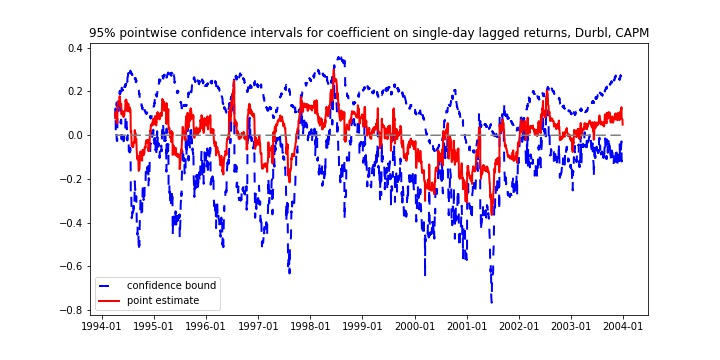
\includegraphics[width=\textwidth]{Durbl/bwunif_pointwiseCIs_CAPM.jpg}
    \caption{Durbl, CAPM}
    \label{fig:1}
  \end{subfigure}
  %
  \begin{subfigure}[b]{0.4\paperwidth}
    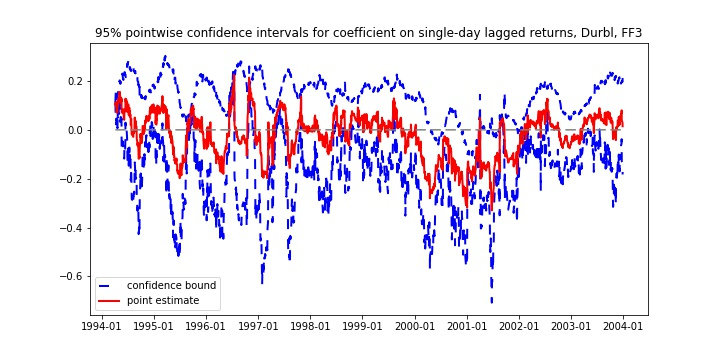
\includegraphics[width=\textwidth]{Durbl/bwunif_pointwiseCIs_FF3.jpg}
    \caption{Durbl, FF3}
    \label{fig:2}
  \end{subfigure}
  %
   \begin{subfigure}[b]{0.4\paperwidth}
    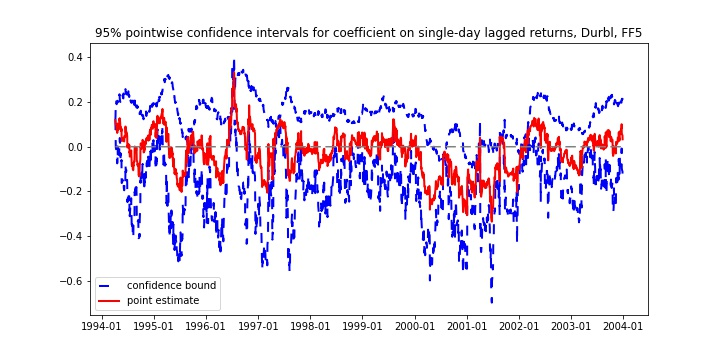
\includegraphics[width=\textwidth]{Durbl/bwunif_pointwiseCIs_FF5.jpg}
    \caption{Durbl, FF5}
    \label{fig:2}
  \end{subfigure}
  \end{figure}

 \newpage
  
  \begin{figure}
  \centering
  \begin{subfigure}[b]{0.4\paperwidth}
    \centering
    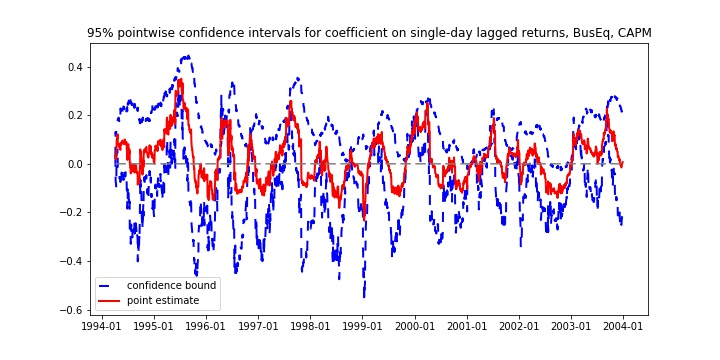
\includegraphics[width=\textwidth]{BusEq/bwunif_pointwiseCIs_CAPM.jpg}
    \caption{BusEq, CAPM}
    \label{fig:1}
  \end{subfigure}
  %
  \begin{subfigure}[b]{0.4\paperwidth}
    \centering
    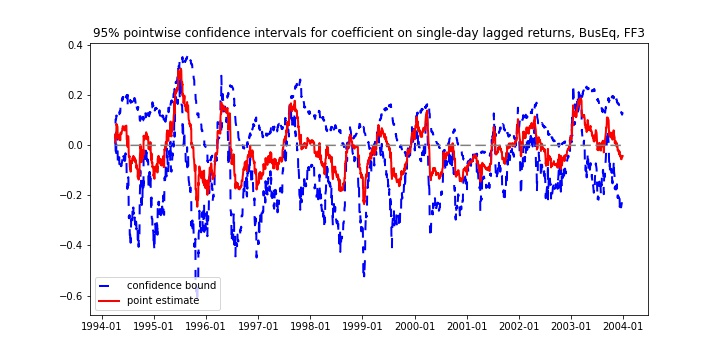
\includegraphics[width=\textwidth]{BusEq/bwunif_pointwiseCIs_FF3.jpg}
    \caption{BusEq, FF3}
    \label{fig:2}
  \end{subfigure}
  %
    \begin{subfigure}[b]{0.4\paperwidth}
    \centering
    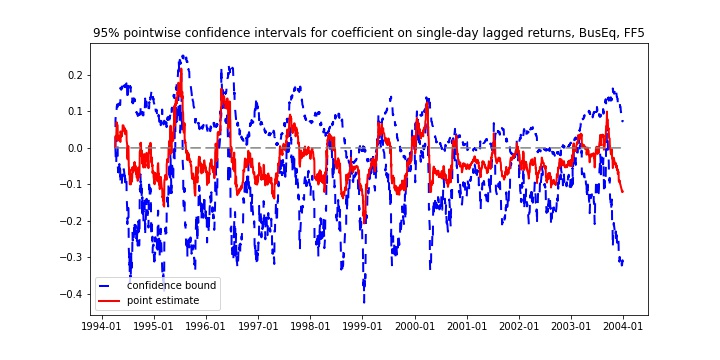
\includegraphics[width=\textwidth]{BusEq/bwunif_pointwiseCIs_FF5.jpg}
    \caption{BusEq, FF5}
    \label{fig:1}
  \end{subfigure}
  %
  \end{figure}
  
  \newpage
  
  \begin{figure}
  \centering
  \begin{subfigure}[b]{0.4\paperwidth}
    \centering
    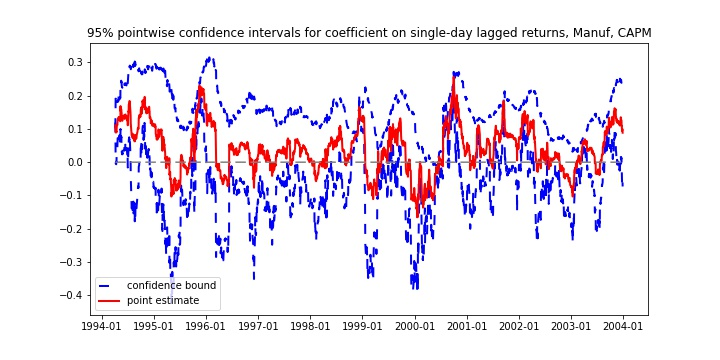
\includegraphics[width=\textwidth]{Manuf/bwunif_pointwiseCIs_CAPM.jpg}
    \caption{Manuf, CAPM}
    \label{fig:1}
  \end{subfigure}
  %
  \begin{subfigure}[b]{0.4\paperwidth}
    \centering
    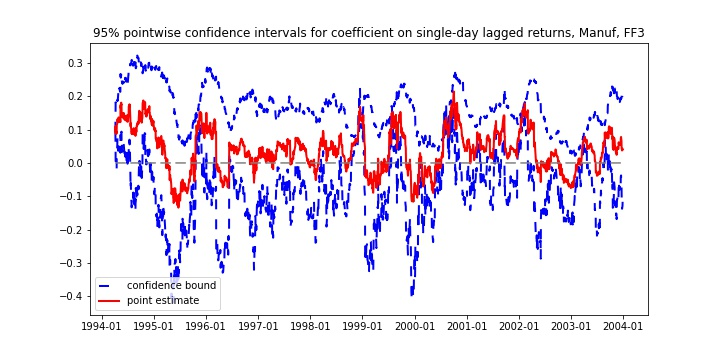
\includegraphics[width=\textwidth]{Manuf/bwunif_pointwiseCIs_FF3.jpg}
    \caption{Manuf, FF3}
    \label{fig:2}
  \end{subfigure}
  %
    \begin{subfigure}[b]{0.4\paperwidth}
    \centering
    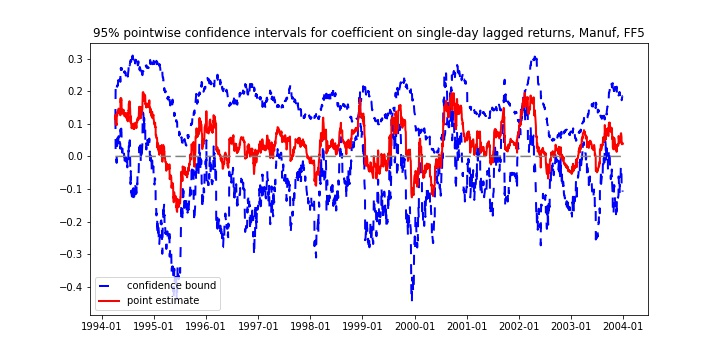
\includegraphics[width=\textwidth]{Manuf/bwunif_pointwiseCIs_FF5.jpg}
    \caption{Manuf, FF5}
    \label{fig:1}
  \end{subfigure}
  %
  \end{figure}
  
  \newpage
  
  \begin{figure}
  \centering
  \begin{subfigure}[b]{0.4\paperwidth}
    \centering
    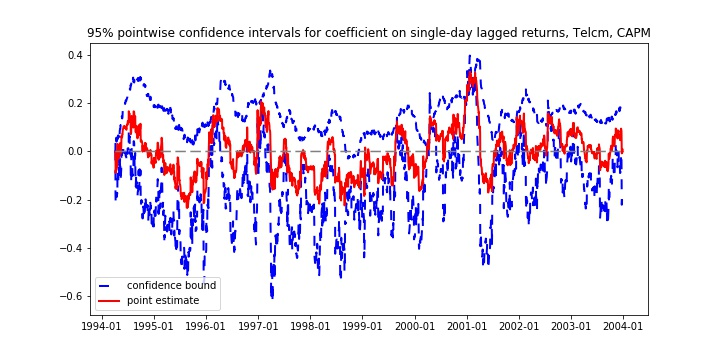
\includegraphics[width=\textwidth]{Telcm/bwunif_pointwiseCIs_CAPM.jpg}
    \caption{Telcm, CAPM}
    \label{fig:1}
  \end{subfigure}
  %
  \begin{subfigure}[b]{0.4\paperwidth}
    \centering
    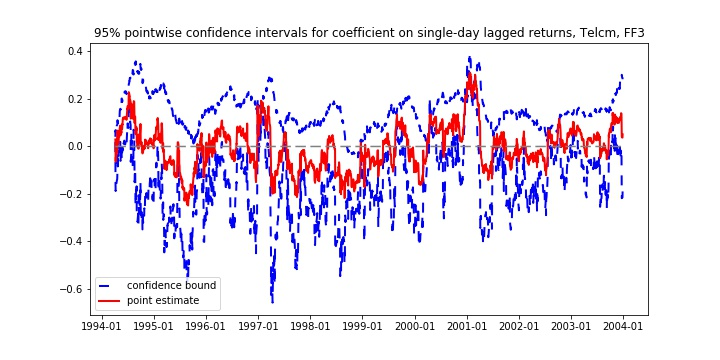
\includegraphics[width=\textwidth]{Telcm/bwunif_pointwiseCIs_FF3.jpg}
    \caption{Telcm, FF3}
    \label{fig:2}
  \end{subfigure}
  %
    \begin{subfigure}[b]{0.4\paperwidth}
    \centering
    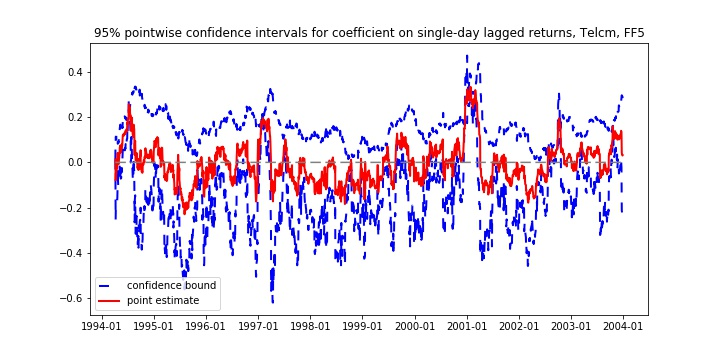
\includegraphics[width=\textwidth]{Telcm/bwunif_pointwiseCIs_FF5.jpg}
    \caption{Telcm, FF5}
    \label{fig:1}
  \end{subfigure}
  %
 \end{figure}
  
  \newpage
  
 \begin{figure}
  \centering
  \begin{subfigure}[b]{0.4\paperwidth}
    \centering
    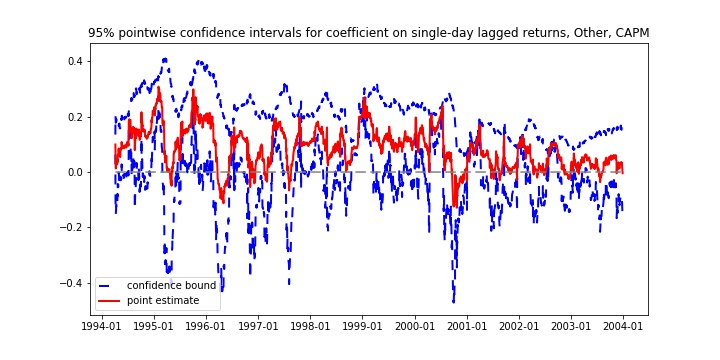
\includegraphics[width=\textwidth]{Other/bwunif_pointwiseCIs_CAPM.jpg}
    \caption{Other, CAPM}
    \label{fig:1}
  \end{subfigure}
  %
  \begin{subfigure}[b]{0.4\paperwidth}
    \centering
    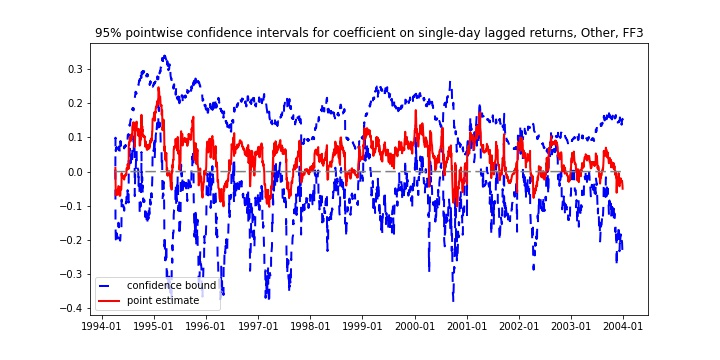
\includegraphics[width=\textwidth]{Other/bwunif_pointwiseCIs_FF3.jpg}
    \caption{Other, FF3}
    \label{fig:2}
  \end{subfigure}
  %
    \begin{subfigure}[b]{0.4\paperwidth}
    \centering
    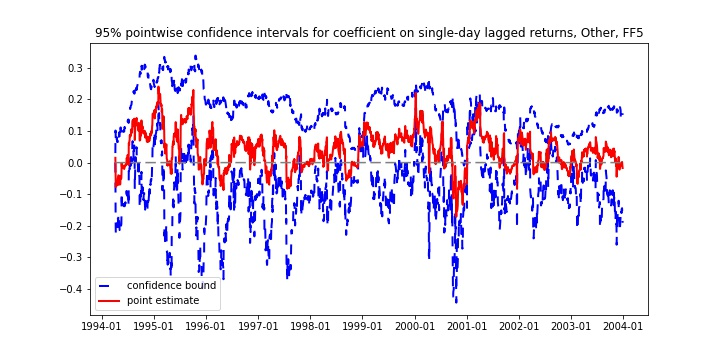
\includegraphics[width=\textwidth]{Other/bwunif_pointwiseCIs_FF5.jpg}
    \caption{Other, FF5}
    \label{fig:1}
  \end{subfigure}
  %
  \end{figure}
        
  \end{landscape}
  \end{document}
  
  